\section{Theory}
\markright{Theory}

A rectifier converts alternating current (AC) into pulsating direct current (DC) using a P-N junction diode, which behaves like a one-way switch \cite{lab03_boylestad2013, lab03_mehta2012}. When forward-biased, the diode conducts once the applied voltage exceeds its barrier potential (about $0.6\text{ V}$ to $0.7\text{ V}$ for silicon). When reverse-biased, it blocks current because of the wide depletion region \cite{lab03_boylestad2013}.

In a half-wave rectifier, a single diode is connected in series with an AC source and a load resistor $R_L$. During the positive half-cycle, the diode is forward-biased and current flows through the load. During the negative half-cycle, it becomes reverse-biased and the output is clipped to zero. The circuit arrangement is shown in Figure \ref{fig:circuit_diagram}.

\begin{figure}[htbp]
  \centering
  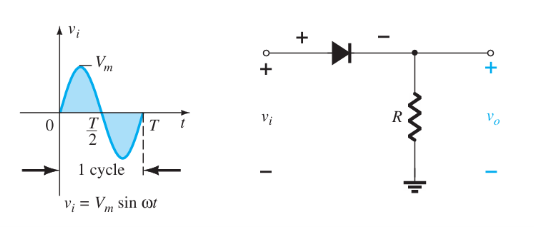
\includegraphics[width=0.6\textwidth]{lab-03/assets/half-wave-rectifier.png}
  \caption{Circuit diagram of a basic diode half-wave rectifier connected to a load resistor $R$ \cite{lab03_boylestad2013}}
  \label{fig:circuit_diagram}
\end{figure}

The output waveform consists of positive pulses separated by zero-voltage intervals. Its shape depends on the input waveform, as shown in Figure \ref{fig:waveforms}.

\begin{figure}[htbp]
  \centering
  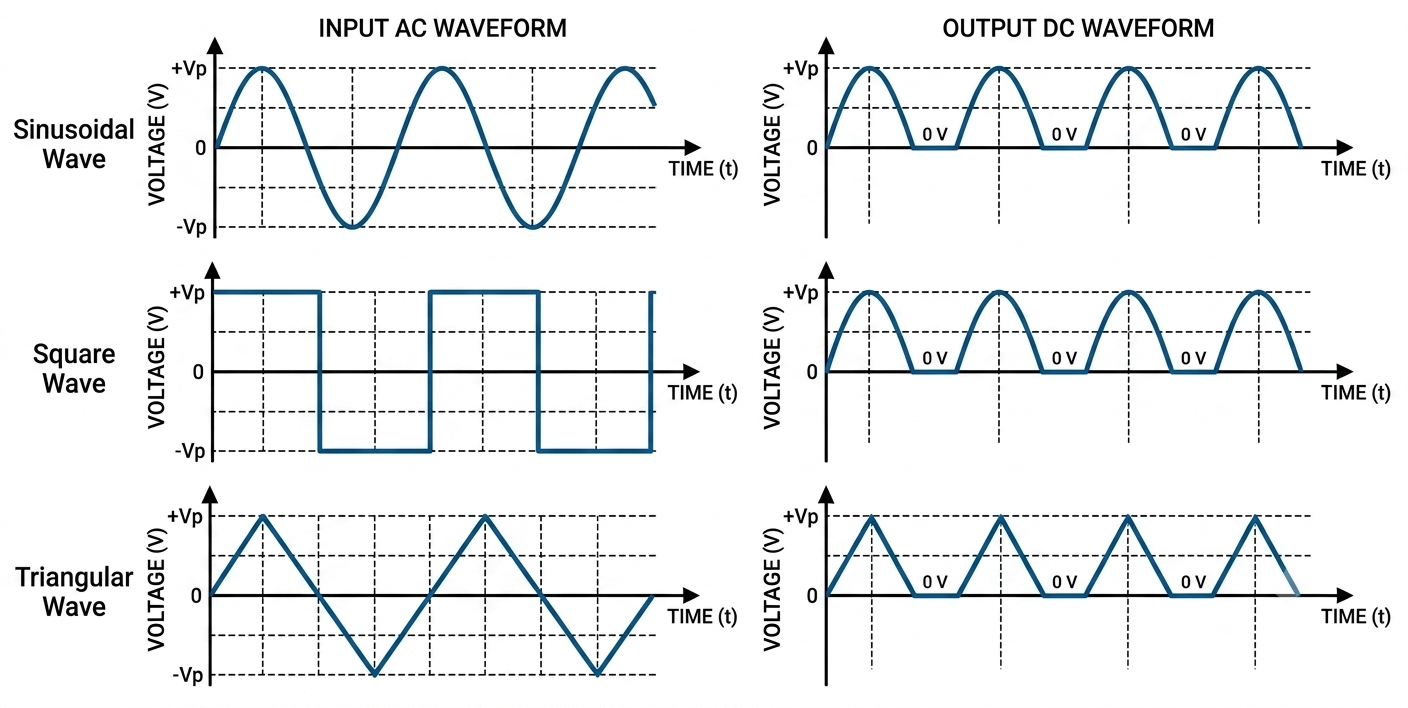
\includegraphics[width=0.88\textwidth]{lab-03/assets/waveforms.png}
  \caption{Comparison of alternating current (AC) inputs and their corresponding pulsating direct current (DC) outputs after half-wave rectification \cite{lab03_gemini2026image}.}
  \label{fig:waveforms}
\end{figure}

The average DC component is given by Eq. \eqref{eq:vdc}, while the ripple content is described by Eq. \eqref{eq:ripple-factor}. The rectification efficiency is expressed by Eq. \eqref{eq:efficiency}. The corresponding relations are:
\begin{equation}
  V_{\text{dc}} = \frac{V_{\text{pp}}}{2\pi}
  \label{eq:vdc}
\end{equation}

The RMS value of the rectified waveform depends on the input waveform shape:
\begin{equation}
  \text{Ripple Factor} = \frac{\sqrt{V_{\text{rms}}^2 - V_{\text{dc}}^2}}{V_{\text{dc}}}
  \label{eq:ripple-factor}
\end{equation}
\begin{itemize}
  \item Square wave: $V_{\text{rms}} = \frac{V_{\text{pp}}}{2}$
  \item Triangular wave: $V_{\text{rms}} = \frac{V_{\text{pp}}}{2\sqrt{3}}$
  \item Sinusoidal wave: $V_{\text{rms}} = \frac{V_{\text{pp}}}{2\sqrt{2}}$
\end{itemize}
\begin{equation}
  \text{Efficiency } (\%) = \frac{P_{\text{dc}}}{P_{\text{ac}}} \times 100\% = \frac{(V_{\text{dc}})^2}{(V_{\text{rms}})^2} \times 100\%
  \label{eq:efficiency}
\end{equation}
